\documentclass[a4paper,11pt]{report}
\usepackage[utf8]{inputenc}
\usepackage[T1]{fontenc}
\usepackage[italian]{babel}
\usepackage{indentfirst}
\usepackage{amsmath}
\usepackage{graphicx}
\usepackage{listings}
\usepackage{color}

\definecolor{mygreen}{RGB}{46,139,87}
\definecolor{myred}{RGB}{165,42,42}
\definecolor{mypurple}{RGB}{160,32,240}
\definecolor{gray}{rgb}{0.5,0.5,0.5}
\definecolor{mauve}{RGB}{255,0,255}
 
\lstset{ %
  language=C,                     % the language of the code
  basicstyle=\ttfamily\footnotesize,           % the size of the fonts that are used for the code
  numbers=left,                   % where to put the line-numbers
  numberstyle=\tiny\color{gray},  % the style that is used for the line-numbers
  stepnumber=1,                   % the step between two line-numbers. If it's 1, each line 
                                  % will be numbered
  numbersep=5pt,                  % how far the line-numbers are from the code
  backgroundcolor=\color{white},      % choose the background color. You must add \usepackage{color}
  showspaces=false,               % show spaces adding particular underscores
  showstringspaces=false,         % underline spaces within strings
  showtabs=false,                 % show tabs within strings adding particular underscores
  frame=single,                   % adds a frame around the code
  rulecolor=\color{black},        % if not set, the frame-color may be changed on line-breaks within not-black text (e.g. commens (green here))
  tabsize=2,                      % sets default tabsize to 2 spaces
  captionpos=b,                   % sets the caption-position to bottom
  breaklines=true,                % sets automatic line breaking
  breakatwhitespace=false,        % sets if automatic breaks should only happen at whitespace
  title=\lstname,                   % show the filename of files included with \lstinputlisting;
                                  % also try caption instead of title
  keywordstyle=\color{mygreen},          % keyword style
  commentstyle=\color{blue},       % comment style
  stringstyle=\color{mauve},         % string literal style
  escapeinside={\%*}{*)},            % if you want to add a comment within your code
}

\title{\bfseries{\Huge{Relazioni di Laboratorio di Fisica Computazionale}}}
\author{\textit {Luca Cassia - [MAT. 728341]}}

\date{Spring 2012}
\begin{document}
\maketitle
\tableofcontents

\chapter{\huge Integrazione Numerica}

\section{Quadrature Gaussiane}
\section{Monte Carlo}
\section{Campionamento d'Importanza}

\chapter{\huge Algoritmo Metropolis}

\lstinputlisting{main/metropolis.c}

\section{L'Oscillatore Armonico Quantistico}
\section{Azione e Termalizzazione}

\begin{figure}[htb]
\centering
\includegraphics[width=\textwidth]{action}
\caption{Azione Euclidea}
\label{fig:action}
\end{figure}

\begin{figure}[htb]
\centering
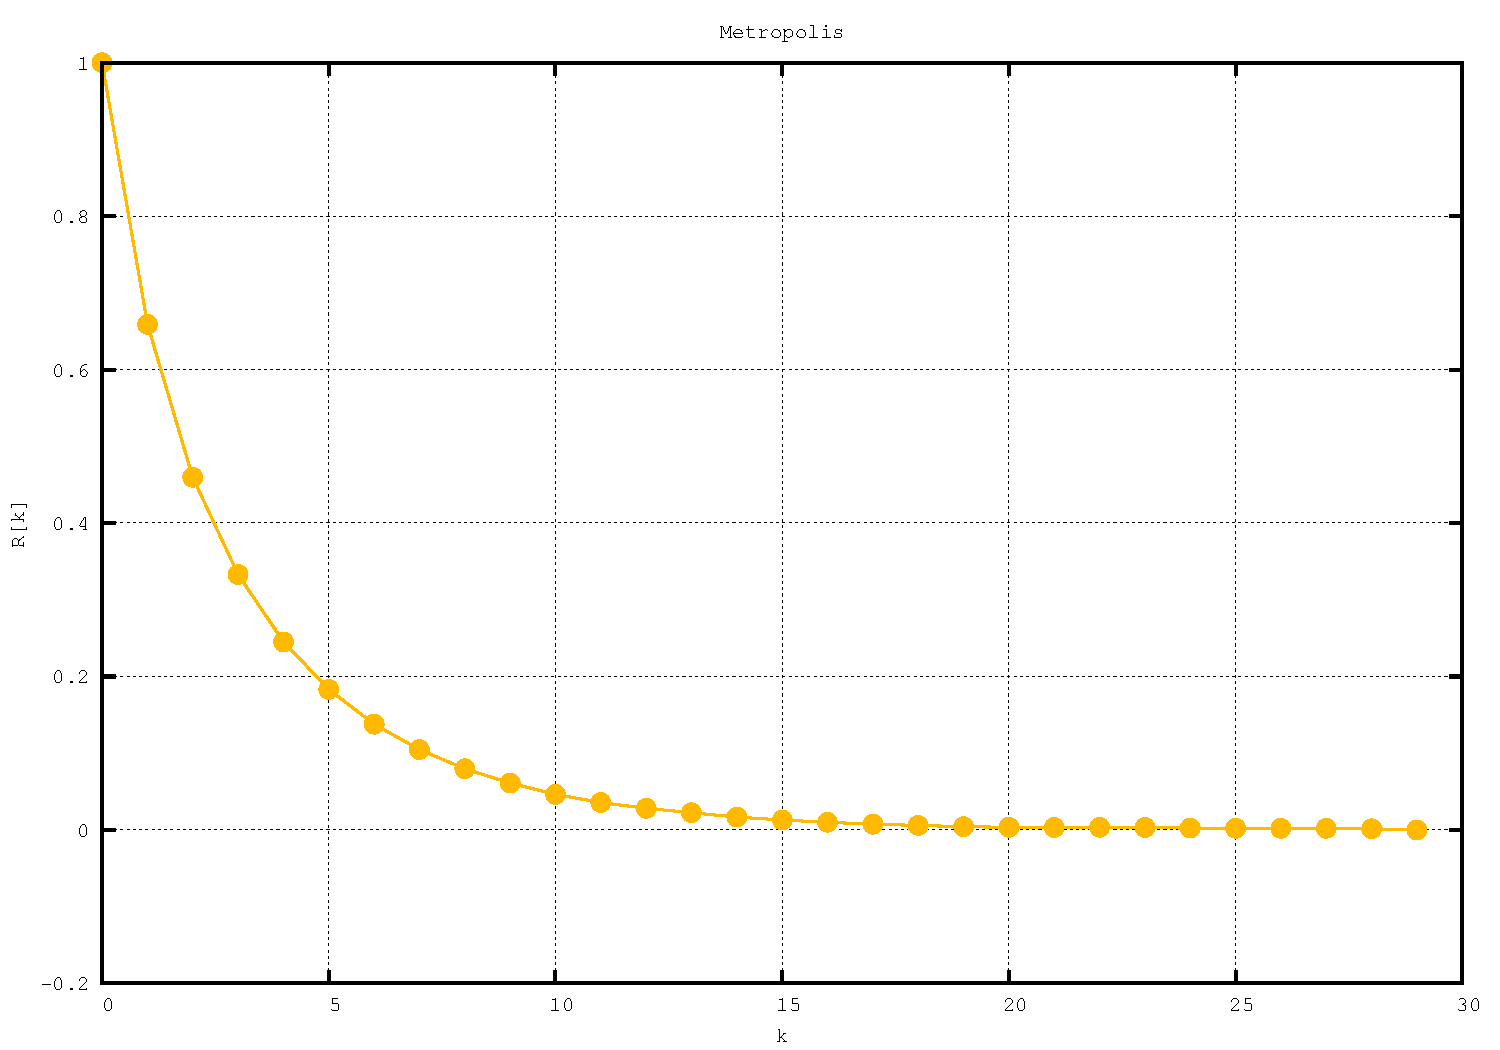
\includegraphics[width=\textwidth]{autocorrelation}
\caption{Autocorrelazione}
\label{fig:autocorrelation}
\end{figure}

\begin{figure}[htb]
\centering
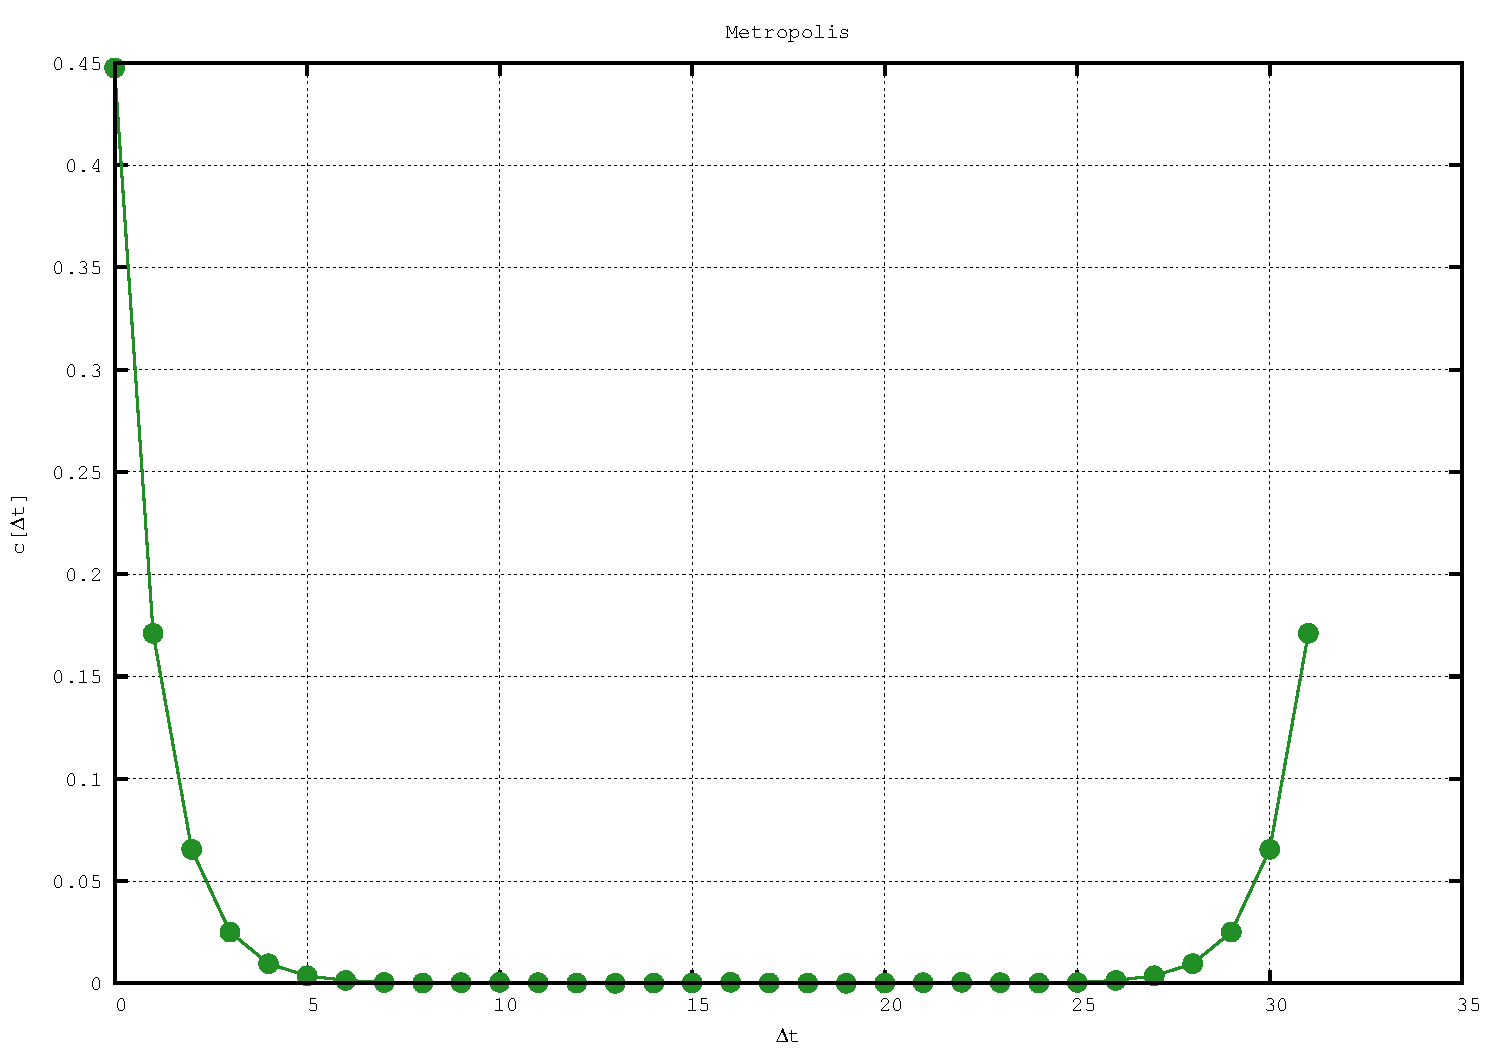
\includegraphics[width=\textwidth]{correlation}
\caption{Correlazione}
\label{fig:correlation}
\end{figure}

\begin{figure}[htb]
\centering
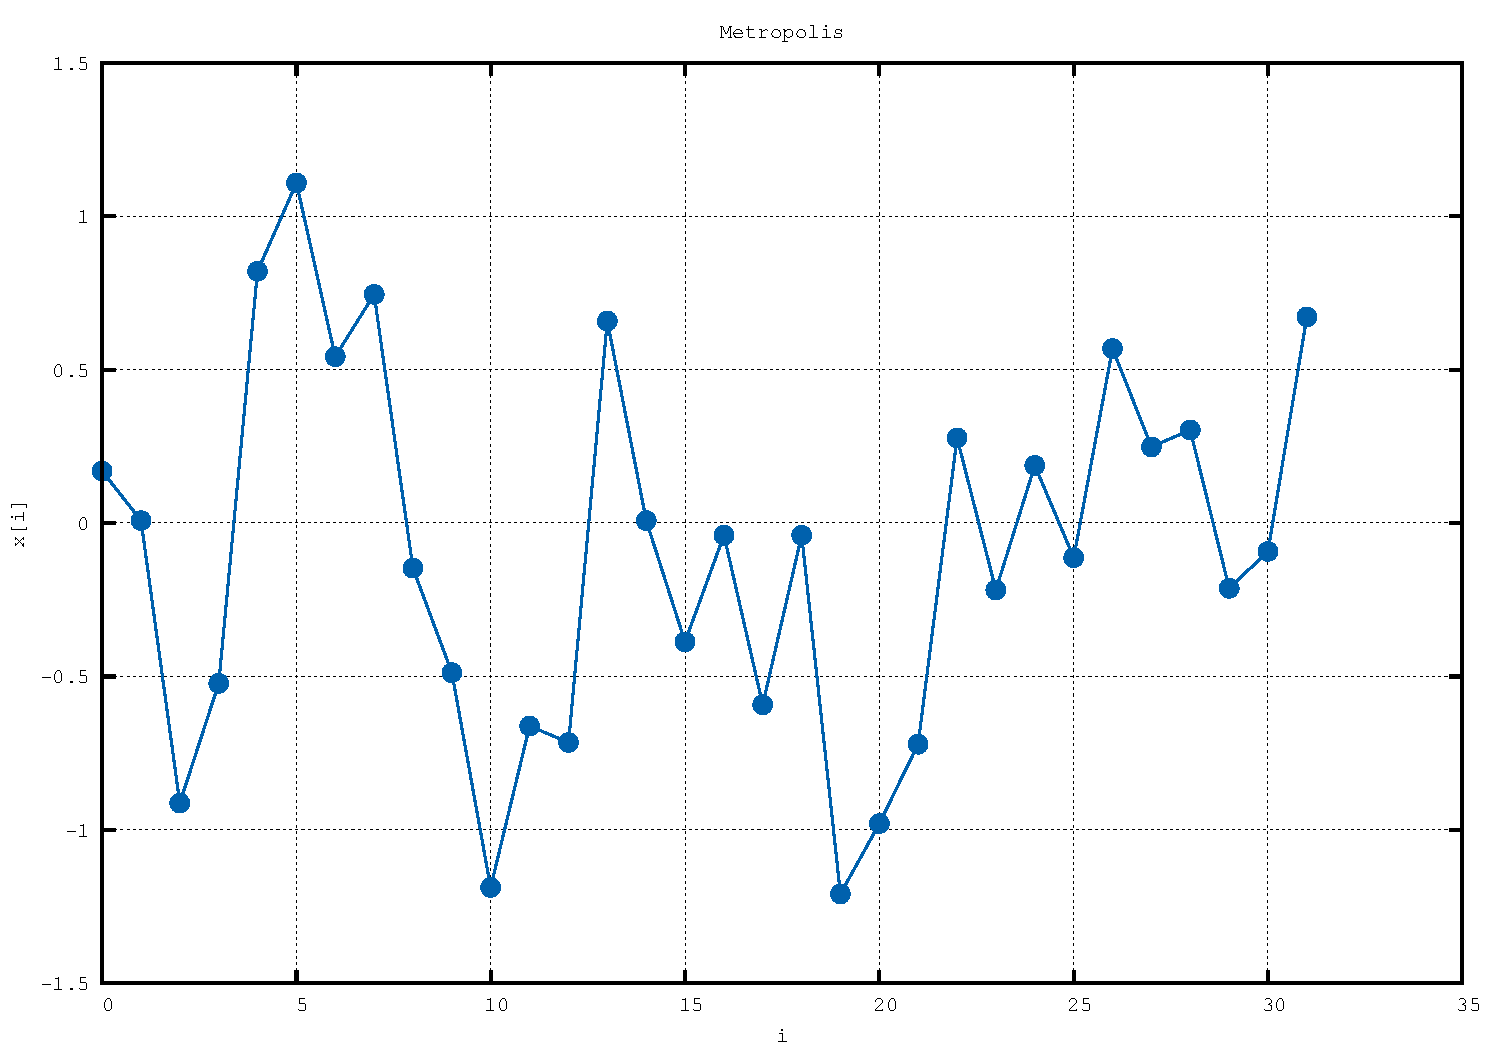
\includegraphics[width=\textwidth]{configuration}
\caption{Configurazione}
\label{fig:configuration}
\end{figure}

\begin{figure}[htb]
\centering
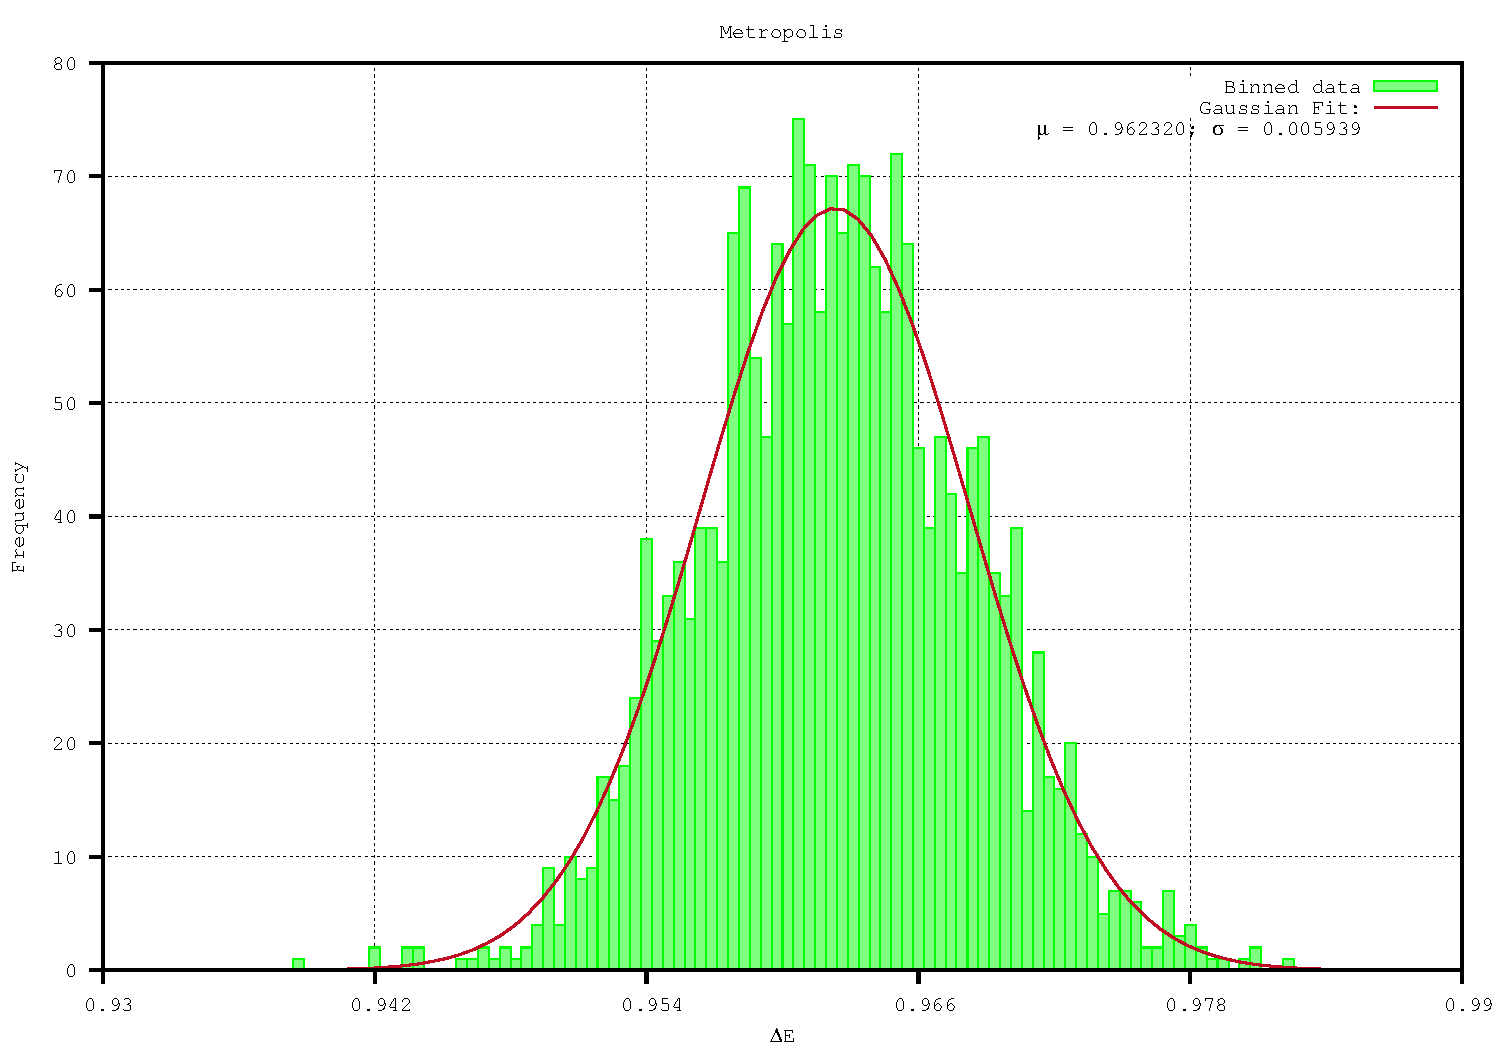
\includegraphics[width=\textwidth]{histogram}
\caption{Istogramma}
\label{fig:histogram}
\end{figure}

\section{Autocorrelazione}
\section{Correlazione}
\section{Calcolo di $\Delta$E}
\section{Calcolo dell'Elemento di Matrice}

\chapter{\huge Metodo Runge-Kutta per Equazioni Differenziali Ordinare}

\section{Il Pendolo Caotico}
\section{Oscillatore di Van Der Pol}
\section{Attrattore di Lorenz}
\section{N-Body Simulation}

\chapter{\huge Altri Metodi per PDE}

\section{Equazioni delle Onde e della Diffusione}
\section{Metodo Implicito ed Equazione di Schr\"{o}dinger}

\end{document}
